\subsection{Insightful limits reveal fundamental behavior}
\label{sec:reason-limits}


Modern deep learning systems are enormous: they regularly involve hundreds of interacting architectural components comprised of hundreds of billions of parameters and trained on trillions of tokens.
With so many interacting degrees of freedom, constructing detailed microscopic theories that track individual parameters in practical systems seems all but hopeless.

Fortunately, complex systems often simplify when approximated as effectively \emph{infinite} in size, revealing simple mathematical structure that remains informative even for the original finite system.
This strategy is well established in statistical and chemical physics: for example, the ideal gas law, $PV = nRT$, is derived in a limit of infinite number of particles (often termed the \textit{thermodynamic} limit) yet accurately describes real parcels of gas of finite volume.
Limits are a central mathematical tool for managing the complexity of deep learning, and their recurring success in doing so provides strong evidence for an emerging theory.

Here we discuss the \textit{limit of infinite width} in detail.
We conclude by mentioning other limits and offering some unifying ideas.


\paragraph{The infinite width limit and the lazy/rich dichotomy.}
The dynamics of a deep neural network often simplify when one takes the number of neurons in each hidden layer to infinity.
Such a limit generally leads to so-called \textit{mean-field} behavior in which we only need to describe the evolution of the neuron population as a whole (as e.g. a probability distribution) and we can ignore what each individual neuron is doing.
However, achieving this limit requires shrinking the initialization scale as width increases to prevent activations in deeper layers from diverging.
The key subtlety in taking the infinite width limit is that the \textit{rate} at which we suppress these initial weights strongly influences the resulting training dynamics, leading to one of two qualitatively distinct limiting behaviors.

\textit{The lazy, kernel, or linearized regime.}
The first forays into the land of infinite width studied only a network's statistics at initialization, not its training dynamics \citep{neal:1996,poole:2016}.
These works found that, in order for the inputs to hidden neurons to neither vanish nor explode as width increases, the parameter size at initialization has to decay as $\text{[width]}^{-1/2}$.
This is not a surprise: it is just the well-known LeCun initialization rule \citep{lecun:1998}, which can be easily derived from the central limit theorem.
Later works that tried naively training the parameters of these infinite-width networks found the surprising fact that the network's \textit{weights and hidden representations} change only negligibly, yet these small changes accumulate to produce substantial changes in the output function.
As a result, the training dynamics are \textit{linear in the parameters} in the sense discussed in \cref{sec:reason-dynamics}, and the evolution of the target function may be expressed entirely in terms of the NTK \citep{jacot2018neural,lee2019wide}.
While a network in this limit is wonderfully analytically tractable, the fact that its hidden representations do evolve only negligibly means that it fails to exhibit \textit{feature learning.}
While the definition of feature learning is much debated (see \cref{openquestion:what_are_features}), all agree that at minimum it requires the network's hidden activations on a given data sample to change from their values at initialization, which does not happen in this limit.
This suggests the NTK infinite-width limit is not the right one to study.
Networks in this linearized regime were later termed ``lazy'' by \citet{chizat2019lazy}.

\begin{figure}
    \centering
    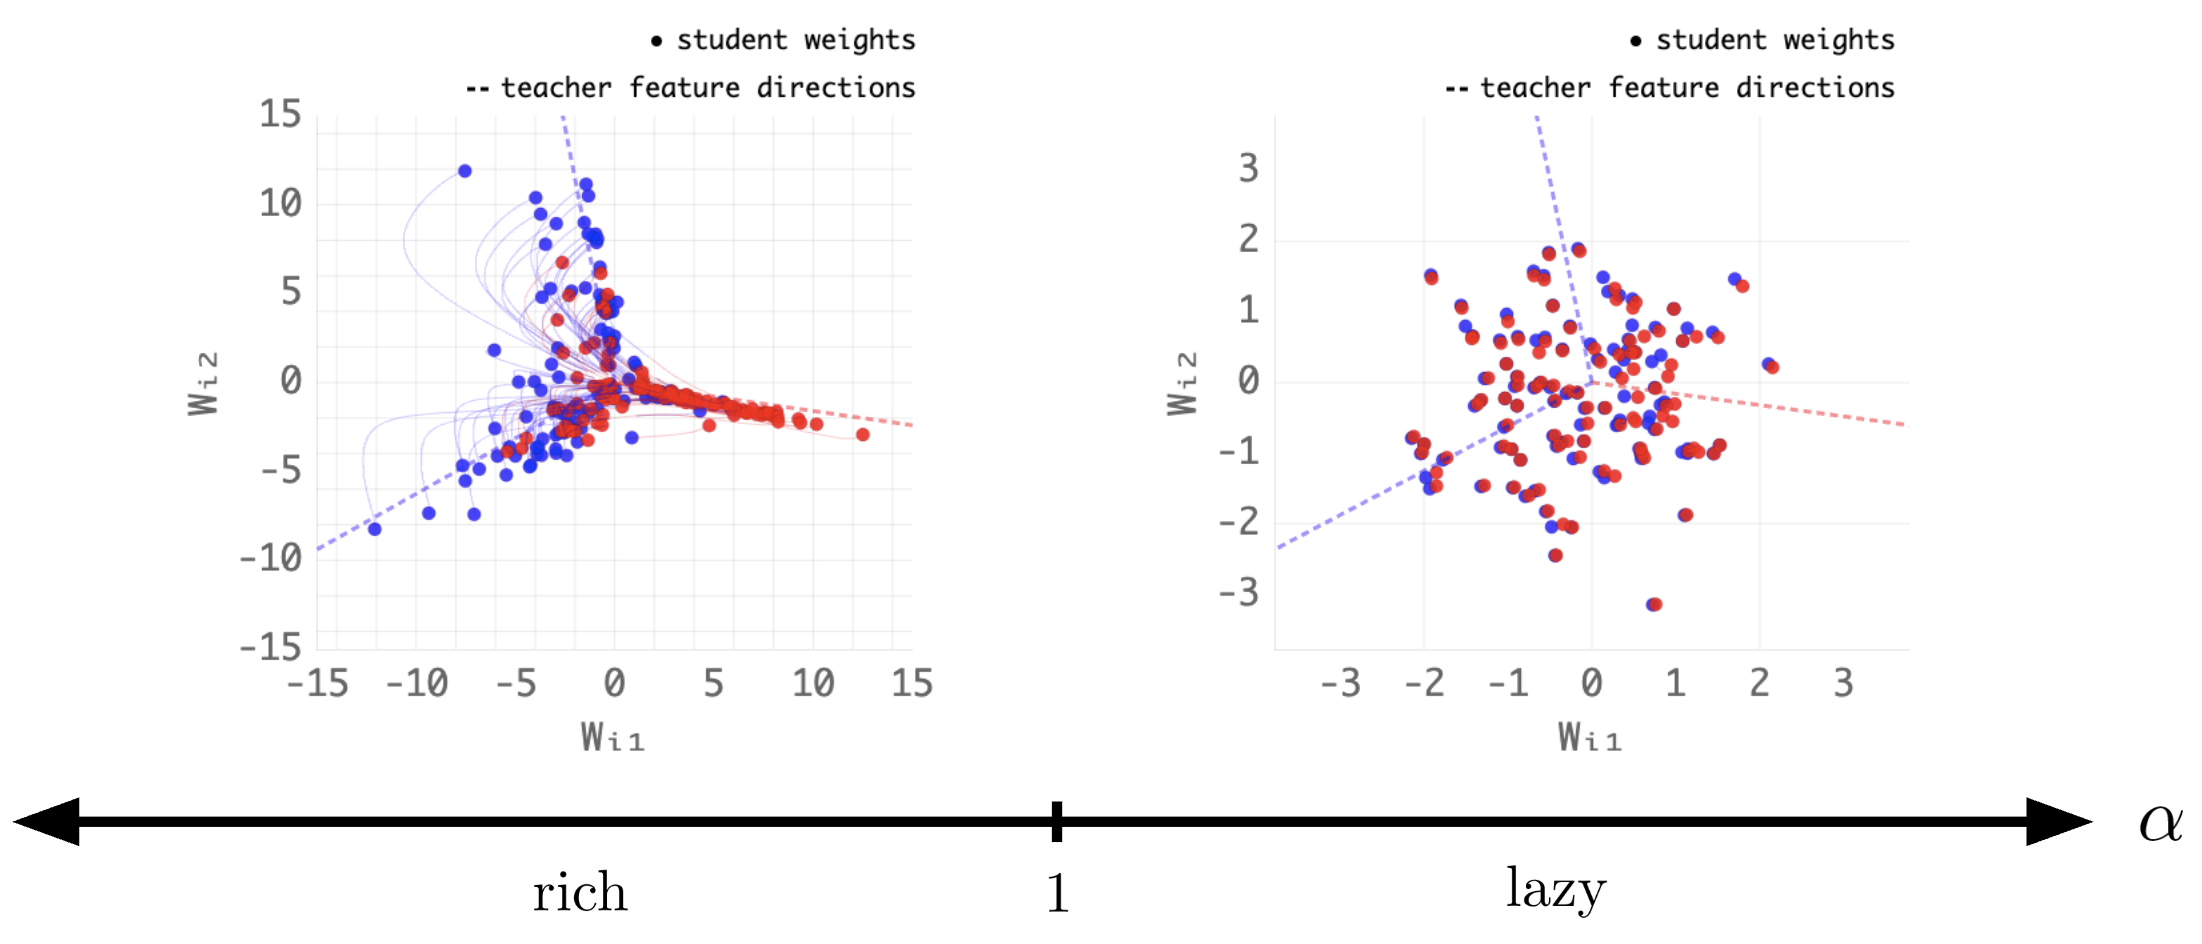
\includegraphics[width=15cm]{figs/limits/lazy_rich_plots.png}
    \caption{
    \textbf{Large and small network output multipliers are sufficient to induce lazy and rich training dynamics.}
    We train a shallow student network $\hat{f}(\vx) = \frac{\alpha}{n} \sum_{i=1}^n a_i \text{ReLU}(\vw_i^\top \vx)$ with width $n = 200$ to match a teacher network $f^*(\vx) = \sum_{i=1}^3 a^*_i \text{ReLU}((\vw^*_i)^\top \vx)$ on two-dimensional input data.
    We plot the training trajectories of the student weights $w_i$ (color denotes $\mathrm{sgn}(a_i)$) against the teacher feature directions.
    \textbf{Left:} with $\alpha = 0.1$, the dynamics are \textit{rich:} the student weights grow significantly and cluster in angle around the teacher feature directions.
    \textbf{Right: } with $\alpha = 30$, the dynamics are \textit{lazy:} the student weights move negligibly during training, even though the loss drops.
    Experiment reproduced from \citet{chizat2019lazy}.
    }
    \label{fig:lazy_vs_rich}
\end{figure}


\textit{The rich, active, or feature-learning regime.}
In answer to this, several authors identified an alternative infinite width limit in which training \textit{does} induce feature learning.
The key insight was essentially to downscale the final-layer weights by a factor of $\text{[width]}^{-1}$, rather than the earlier $\text{[width]}^{-1/2}$, thereby forcing the network weights to change more to compensate.%
\footnote{The lazy vs. rich dichotomy is conceptually similar to elastic vs. plastic deformation in materials. A material will deform linearly in response to a small force, and its internal atomic structure will not change. In response to a larger force, it will deform nonlinearly, and its internal structure changes.}
While this makes the function trivial at initialization (at infinite width it is uniformly zero), it can still grow nontrivially during training, changing by an order-one amount upon each gradient step.

This downscale-the-network-output idea first appeared in the shallow ``mean-field networks'' of \citet{mei2019mean}, \citet{rotskoff2018parameters}, and \citet{chizat2018global}.
\citet{geiger2020disentangling} and \citet{yang2021tensor} found that this idea also works for networks of arbitrary depth, bundling the resulting hyperparameter scaling factors together into the celebrated ``Maximal Update Parameterization'' discussed in \cref{sec:reason-hps}.
It is now widely accepted that infinite-width neural networks can learn features.

Wide networks in this ``rich'' regime display a huge range of interesting behaviors that their lazy counterparts do not.
The most significant is certainly that the hidden features of these networks change over time, adapting to the structure in the input data, altering the internal geometry of hidden representations over the course of training \citep{bordelon2022self}.
Subpopulations of neurons specialize, learning to attend to different features latent in the data \citep{aubin2018committee, goldt2019dynamics, ren2025emergence}.
For instance, in tasks where the optimal predictions involve low-dimensional subspaces of high dimensional data, the distribution over first layer weights evolves to amplify weights in the subspace of interest \citep{mei2018mean, abbe2022merged, moniri2023theory, cui2024asymptotics, defilippis2025scaling, erba2025nuclear, montanari2026phase}.
When the scale of the initialization is made even smaller, they often show the greedy low-rank bias discussed in \cref{sec:reason-dynamics}, acquiring some components of the task before others \citep{saxe2015deep,atanasov2021neural,atanasovoptimization}.%
\footnote{
There is also a well-developed line of work studying the signatures of feature learning in large-width networks from a \textit{Bayesian} perspective.
Naively, infinite-width networks have simple Bayesian statistics given by Gaussian processes \citep{lee2017deep}, which is analogous to the ``lazy'' limit of conventionally-trained networks.
This view treats this Gaussian process limit as a solvable reference point \citep{cohen2021learning,lavie2024towards} and then reintroduces finite width, using mean-field and variational techniques to characterize aspects of feature adaptation to data \citep{cohen2021learning,seroussi2023separation,rubin2023grokking,rubin2025kernels,rubin2025mitigating}.
One may also induce feature learning by rescaling the total likelihood (see e.g. \citet{yang2023theory}), which is analogous to the final-layer downscaling which gives the rich limit in conventional training.
}


The lazy–rich dichotomy, and its dependence on initialization scale, emerged as a central finding of infinite-width analyses.
Subsequent work has shown that analogous behavior appears even at finite width: scaling down the network output promotes feature learning, pushing models toward the rich regime, whereas increasing the output scale tends to linearize training dynamics and induce lazy behavior \citep{chizat2019lazy}.
This sensitivity to initialization scale connects to a broader literature on inductive bias, where seemingly small changes to the learning setup can steer training toward fundamentally different solution classes \citep{maennel2018gradient,woodworth2020kernel}.
\cref{fig:lazy_vs_rich} illustrates how the same finite network, trained with different output scalings, can exhibit either lazy or rich learning dynamics.




\paragraph{The infinite depth limit and other hyperparameter limits.}

As with infinite width, one can arrive at a stable infinite depth limit of a deep residual network by downscaling the contribution of each layer so the residual stream does not blow up.
Here, too, there are different limiting behaviors depending on the size of this downscaling factor: suppressing each layer by a factor of $\text{[depth]}^{-1}$ results in limiting dynamics in which the residual stream changes smoothly over depth \citep{bordelon2024infinite, chizat2025hidden, chaintron2026resnets} (reminiscent of Neural ODEs \citep{chen2018neural}) while suppressing each layer by a factor of $\text{[depth]}^{-1/2}$ results in limiting dynamics in which the residual stream diffuses as if driven by a stochastic differential equation \citep{bordelon2023depthwise, yang2023depth}.
Networks in these two limits converge to qualitatively different solutions in realistic architectures such as transformers \citep{dey2025don}.
It is not yet clear which is the more important limit to study.



Some deep learning architectures admit size limits other than those of large width or large depth. Instead of increasing size or total number of distinct feedforward layers, one can also analyze the infinite limits of recurrent architectures using similar mean-field ideas \citep{clark2026structure, bauer2026unified}. State-of-the-art transformer models include more expressive constituent blocks such as multi-head self-attention layers and mixture-of-expert multi-layer perceptrons. These layers have multiple scaling directions including head count, head size, and context length for attention \citep{hron2020infinite,bordelon2024infinite} and expert count, expert size, and sparsity for mixture-of-expert models \citep{pioromu2025moes,jiang2026hyperparameter}.
Clarifying the interplay of different infinite limits in these models is important to making contact with modern practice and to disentangle various hyperparameters related to initialization and optimization (see Section \ref{sec:reason-hps}).

Lastly, most optimization hyperparameters have an associated limit.
As the batch size approaches infinity, we reach population gradient descent.
As we take learning rate to zero, we recover gradient flow.
If we add an infinitesimal weight decay and take training time to infinity, we first optimize the loss to convergence, then perform parameter norm minimization conditioned on the final value of the loss.
We discuss how to understand the corrections induced by having finite values for some of these hyperparameters in \cref{sec:reason-hps}.


\paragraph{Joint scaling limits.}

Sometimes scaling limits in multiple variables ($\nu_1,\nu_2$) play nicely, in the sense that $\displaystyle \lim_{\nu_1 \to \infty}\,\lim_{\nu_2 \to \infty}$ gives the same result as
$\displaystyle \lim_{\nu_2 \to \infty}\,\lim_{\nu_1 \to \infty}$.
For example, the infinite width and depth limits in residual networks usually commute in this way, so long as one takes a sensible parameterization \citep{hayou2023width}.
However, in many theoretical machine learning settings, different scaling dimensions do not commute, and the limiting behavior could depend on a limiting ratio $\nu_2 / \nu_1$.
Such joint/proportional scaling limits are common in random matrix theory: for example, consider the SVD of a random matrix with $P$ rows and $N$ columns with $N,P \to \infty$ with $P/N$ held constant.
In machine learning theory, neural networks trained with random data can often be described by a joint scaling limit where both the dataset size and parameter count are taken to infinity, but one or more of the \textit{ratios}
$\frac{\text{[data]}}{\text{[input dim]}}$, $\frac{\text{[data]}}{\text{[width]}}$, or $\frac{\text{[data]}}{\text{[parameters]}}$
is a finite value \citep{seung1992statistical,saad1995exact,zdeborova2016statistical,li2021statistical,maillard2024bayes,martin2024impact,barbier2025statistical}.
This joint scaling is likely necessary in the study of \textit{compute-optimal neural scaling laws} where the training horizon (i.e. dataset size) is scaled linearly with the total parameters \citep{hoffmann:2022-chinchilla} and to theoretically characterize hyperparameter transfer phenomena \citep{bordelon2025deep}. These joint (data \& model size) limits are potentially important as infinite parameter limits at fixed dataset size are capable of perfect interpolation and do not capture scaling law behaviors across model sizes (see Section \ref{sec:reason-measurable}).
Other well-studied joint scaling quantities include the ratio
$\frac{\text{[width]}}{\text{[depth]}}$
in non-residual networks \citep{hanin2019finite, li2022neural, noci2023shaped, hanin2025global}, the ratio
$\frac{\text{[learning rate]}}{\text{[output multiplier]}}$
in the rich regime \citep{atanasovoptimization}, and the ``SGD noise temperature''
$\frac{\text{[learning rate]}}{\text{[batch size]}}$ \citep{mandt2017stochastic,jastrzkebski2017three}.

\paragraph{The Discretization Hypothesis.}
Overall, the widespread use of limits to manage the complexity of deep learning reflects a recurring theme across scientific disciplines: appropriate asymptotic perspectives often render otherwise intractable systems analytically tractable.
Many theorists share a heuristic belief that most practical neural networks can be understood as noisy, finite approximations to models of infinite size.%
\footnote{Works studying finite-size corrections to infinite limits include \citep{hanin2019finite,roberts2022principles, zavatone2021asymptotics, segadlo2022unified,bordelon2023dynamics, glasgow2025propagation}.}
By analogy, one numerically solves a partial differential equation by discretizing over space and time, and the finer the discretization, the smaller the numerical error from the desired continuum process.
This is very possibly also true of deep neural networks, with width and depth taking the place of space and time.
Other finite hyperparameters, such as the learning rate, batch size, and dataset size, might also be understood in this way.

We might call this belief the \textit{Discretization Hypothesis.}
While it has yet to be made precise or proven (see \cref{openquestion:discretization}), this hypothesis has implicitly underpinned much important work, and little in the analytical study of large models makes sense without it.

The Discretization Hypothesis amounts to the statement that finite-size corrections from limits typically worsen performance while saving costs in data, time, memory, and compute.
Showing that these finite-size effects deliver a general benefit that cannot be achieved any other way would falsify this hypothesis.
